%! Author = ia
%! Date = 4/22/22

% Preamble
\documentclass[11pt]{article}

% Packages
\usepackage{amsmath}

% Document
\begin{document}

	% \section{\normalsize{Comparing Models and Empirical Data}}
	% .. re: Canonical Emission Rate

	\clearpage

	\textbf{Where is the hump?}

	The empirical data for Ethereum Classic shows a `hump` which is not visible in the
	procedurally sampled Poisson distribution values.

	\subsection{\normalsize{Network latency ($\eta$)}}

	We propose that an explanation can be made for this unexpected shape
	by a consideration of network latency.

	\vspace{5mm}
	\begin{proposition}
		Latency exists.
	\end{proposition}

%The material existence of network latency is irrefutable under current physical models of the world.
%Information cannot travel faster than the speed of light, which is finite.
%The networks in question assume the transmission of messages (information), and thus, this takes time.
	Latency is the time required for message transmission.

	The production of any block depends on the observation of the block it will be appended to, its parent.
	A miner can only begin mining block $B_{i=n}$ after observing block $B_{i=n-1}$.

	Arbitrarily defining network latency as a constant $\eta=3$ seconds allows us
	to produce a revised histogram of expected Poisson event intervals.

	\begin{figure}[tph]
		\centering
		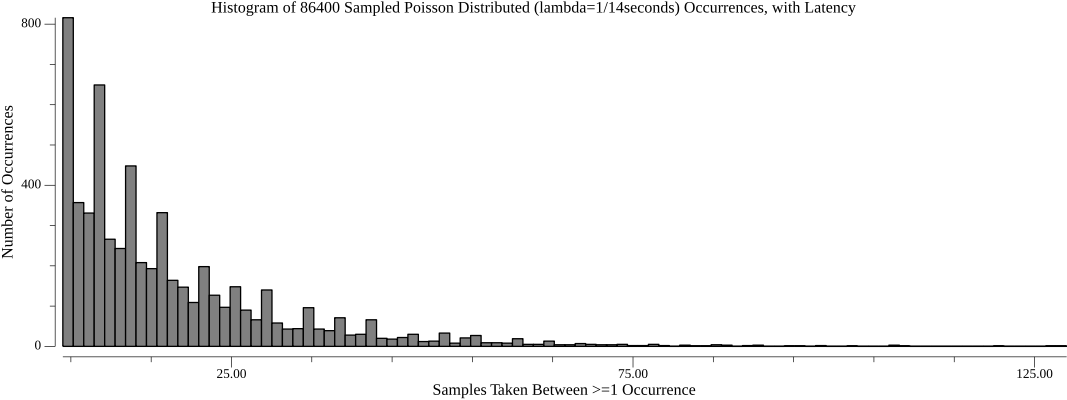
\includegraphics[width=1.0\textwidth]{go-block-step/out/vis_poisson_samples_eventintervals_latencynaive_hist.png}
		\caption{
			Procedurally generated events $k \geq 1$ interval samples from a Poisson process
			with $\lambda = \frac{1}{14}$, with a sample size of 86400.
			Every interval is increased by $\eta=3$ seconds.
			Clearly, this general application of latency is insufficient.
			The shape is unchanged; only the domain is shifted by $3$.
		}
	\end{figure}

	\vspace{5mm}
	\begin{proposition}
		Latency is heterogenous.
	\end{proposition}

	If we assume there exist $m$ miners on the network, and that each miner
	controls $\frac{1}{m} \times \networkHashrate$, we can estimate the rate of the
	same miner producing blocks $B_{i=n}$ and its child $B_{i=n+1}$ as
	$\frac{1}{m}$.
	When a miner produces both the Parent and Child blocks, the $\eta$ value for
	that interval should approach $0$; where time of program execution alone is
	considered relative to the aggregate time of program execution plus network
	transmission duration.
	We arbitrarily define $m=8$, and, accounting for this probability, produce
	Figure 23.

	\begin{figure}[tph]
		\centering

		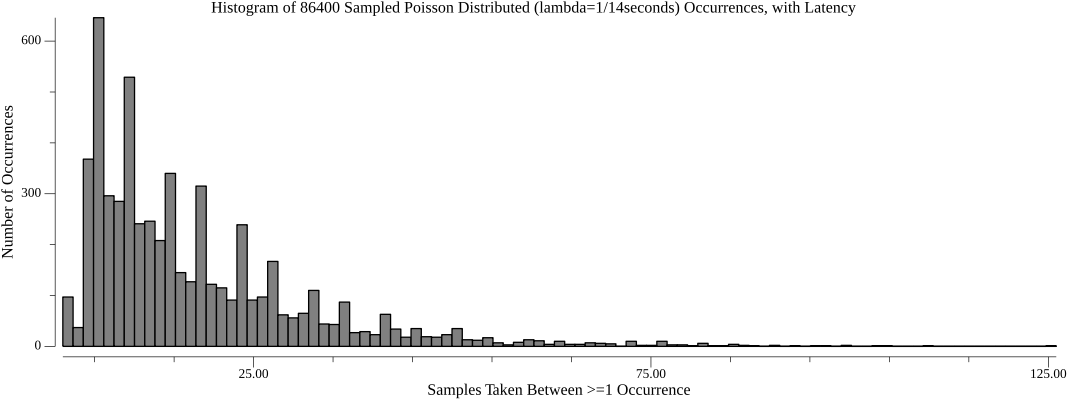
\includegraphics[width=1.0\textwidth]{go-block-step/out/vis_poisson_samples_eventintervals_latencysamesame_hist.png}
		\caption{
			Procedurally generated events $k \geq 1$ interval samples from a Poisson distribution
			with $\lambda = \frac{1}{14}$, with a sample size of 86400.
			Every interval is increased by $\eta=3$ for approximately
			$1-\frac{1}{8}$ of the intervals.
		}
	\end{figure}

	Though still naive, we have found a hump.

	\vspace{5mm}
	\begin{proposition}
		Latency's heterogeneity depends on miner hashrate. %% , and thus, the $\frac{1}{m}$ model is inaccurately simplistic.
	\end{proposition}

	We assume that miner hashrate for the Ethereum network is unevenly distributed.
	This assumption causes our estimation above of Parent/Child same-miner events
	as $\frac{1}{m}$ to be inaccurate.
	Under this theoretical model, we do not pursue further revisions for this
	approximation.

	\vspace{5mm}
	\begin{proposition}
		Latency may be optional.
	\end{proposition}

	If latency is defined as the time between transmission and reception of a
	message, it attributes should be mostly attributable to physical or
	otherwise 'external' limitations.\nolinebreak\footnote{
		e.g Cable size, net neutrality (or lack thereof).
	}

	However, if we were instead to define latency as the time between the availability
	of the message (to the transmitor) and the time of message reception,
	a new variable arises: delay.

	By creating a delay on purpose, a miner gives themselves a head-start
	on the mining of a next block. They postpone the transmission of their message,
	stalling the game for the rest of the network. While this strategy can benefit
	the miner, it comes with the risk that another miner may produce (or have
	produced) a competitor block in this interval reducing their chances of success.

	On this topic, the reader should reference Eyal and Sirer\footnote{TODO}, who
	show that large-hashrate miners (ie. 25\%, 33\%, etc.) can be reasonably
	expected to demonstrate this behavior, and with it, a block emission
	rate superlinear to their hashrate ratio. They propose network bifurcation
	(via a simulated coin-toss) as a network protocol strategy for mitigating
	this incentive.

	\begin{figure}[tph]
		\centering

		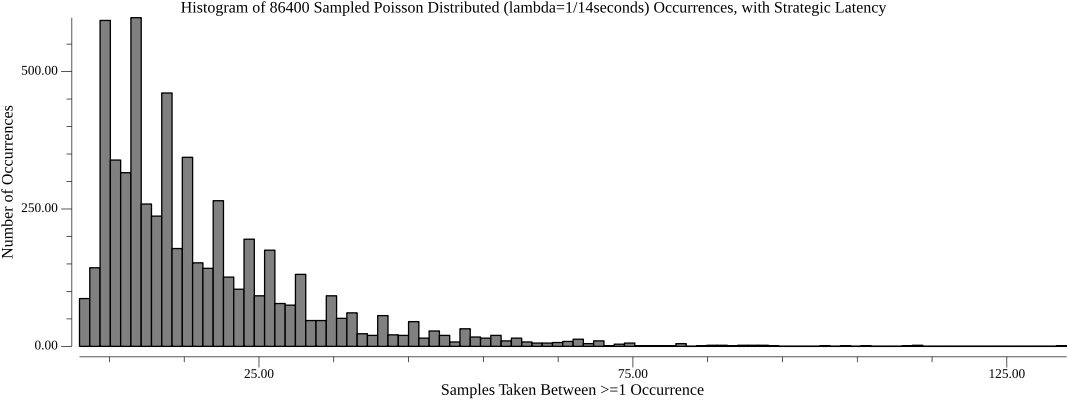
\includegraphics[width=1.0\textwidth]{go-block-step/out/vis_poisson_samples_eventintervals_latencysamesamestrat_hist.png}
		\caption{
			Procedurally generated events $k \geq 1$ interval samples from a Poisson distribution
			with $\lambda = \frac{1}{14}$, with a sample size of 86400.
			Every interval is increased by $\eta=3 + \frac{1}{8} \times \mathrm{interval_{\Delta}}$ seconds for approximately
			$1-\frac{1}{8}$ of the intervals.
			This represents a loose event interval model including selfish miner delays.
		}
	\end{figure}

%% Let's compare them!

%begin{figure}[tph]
%\centering
%
%
%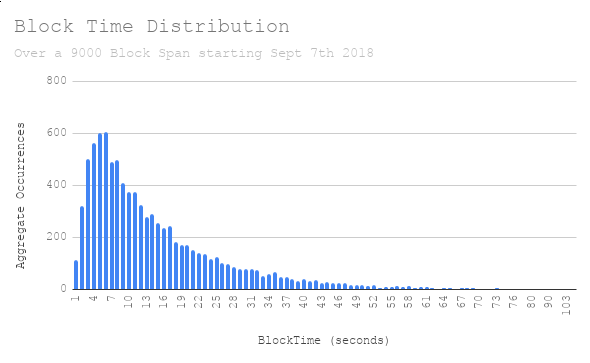
\includegraphics[width=1.0\textwidth]{vis_data_blockinterval_distribution.png}
%\caption{
%    Exemplary block interval data for
%    Ethereum.\footnote{https://ethresear.ch/t/deep-dive-into-current-pow-difficulty-
%    adjustment-algorithm-and-a-possible-alternative/5267}
%}
%\end{figure}


\end{document}